\documentclass[english]{elsarticle}
\usepackage[T1]{fontenc}
\usepackage[utf8]{inputenc}
\usepackage[a4paper]{geometry}
\geometry{verbose}
\usepackage{amsthm}
\usepackage{amsmath}
\usepackage{amssymb}
\usepackage{graphicx}
\usepackage{esint}

\makeatletter

%%%%%%%%%%%%%%%%%%%%%%%%%%%%%% Textclass specific LaTeX commands.
  \theoremstyle{definition}
  \newtheorem{defn}{\protect\definitionname}
  \theoremstyle{plain}
  \newtheorem{prop}{\protect\propositionname}
\theoremstyle{plain}
\newtheorem{thm}{\protect\theoremname}

%%%%%%%%%%%%%%%%%%%%%%%%%%%%%% User specified LaTeX commands.


\usepackage{amsthm}\usepackage{bbm}\usepackage{tabularx}



\usepackage{times}%\usepackage{subfloat}
%\usepackage{subfig}


\def\d{\mathrm{d}}
\def\dmu{\mathrm{d}\mu}
\def\fD{\mathcal{D}}
\def\Rset{\mathbb{R}}
\def\X{\mathcal{X}}
\def\Y{\mathcal{Y}}
\def\un{\mathbbm{1}}
\def\e{\operatorname{e}}
\def\W{\operatorname{W}}
\def\ext{\operatorname{ext}}
\def\sech{\operatorname{sech}}
\def\arsech{\operatorname{arsech}}
\def\argtanh{\operatorname{argtanh}}
%
\newcommand{\Esp}[1]{\mathbb{E}\left[ #1 \right]}

\newtheorem{definition}{Definition}
\newtheorem{proposition}{Proposition}

%%%

\def\ps@pprintTitle{%
  \let\@oddhead\@empty
  \let\@evenhead\@empty
  \def\@oddfoot{\reset@font\hfil\thepage\hfil}
  \let\@evenfoot\@oddfoot
}

\makeatother

\usepackage{babel}
  \providecommand{\definitionname}{Definition}
  \providecommand{\propositionname}{Proposition}
\providecommand{\theoremname}{Theorem}

\begin{document}
\global\long\def\d{\mathrm{d}}


\global\long\def\dmu{\mathrm{d}\mu}
 

\global\long\def\fD{\mathcal{D}}


\global\long\def\Rset{\mathbb{R}}


\global\long\def\X{\mathcal{X}}


\global\long\def\un{\mathbbm{1}}


\global\long\def\Esp#1{\mathbb{E}\left[ #1 \right]}


\global\long\def\e{\operatorname{e}}


\global\long\def\W{\operatorname{W}}


\global\long\def\ext{\operatorname{ext}}


\global\long\def\sech{\operatorname{sech}}
\global\long\def\arsech{\operatorname{arsech}}
 \global\long\def\argtanh{\operatorname{argtanh}}



\title{T'aurais pas une entropie?}


\author{by jfb \& co \date{} }
\begin{abstract}
  Where  we  show  that it  is  possible  to  derive  new entropies  yielding  a
  particular specified  maximum entropy distribution. There  are (probably) many
  errors  --I  hope  not  fundamental  but  is  is  possible;  (certainly  many)
  approximations,   typos,   maths   and   language   mistakes.Suggestions   and
  improvements will be much appreciated.
\end{abstract}
\maketitle
% -------------------- MaxEnt -------------------- %



\section{Maximum entropy distributions}

\label{sec:MaxEnt}

Let $f$ be a probability distribution  defined with respect to a general measure
$\mu$ on a set $\X$ and ${\displaystyle S[f]=-\int_\X f(x)\log f(x) \dmu(x)}$ be
the  Shannon  entropy  of  $f$.   Subject  to $n$  moment  constraints  such  as
$\Esp{T_i(x)} = t_i,  i=1,\ldots,n$ and to normalization, it  is well known that
the maximum entropy distribution lies within the exponential family
\[
f_X(x) = \exp\left( \sum_{i=1}^n \lambda_i T_i(x) + \lambda_0 \right).
\]
In order  to recover  known probability distributions  (that must belong  to the
exponential family), it is then sufficient  to specify a set of functions $T_i$.
This has been used by many authors.  For instance, the gamma distribution can be
viewed as a  maximum entropy distribution if one knows the  moments $\Esp X$ and
$\Esp{\log(X)}$.  In  order to find  maximum entropy distributions  with simpler
constraints or distributions  outside of the exponential family,  it is possible
to  consider  other entropies,  which  is  discussed  below. This  problem  find
interests in goodness-and-fit tests based on maximum entropy principle.


% -------------------- Max (h,phi)-Ent -------------------- %

\section{Maximum $(h,\phi)$-entropy distributions}
\label{sec:MaxPhiEnt}


% ---------- Definition & MaxEnt solutions

\subsection{Definition and maximum $(h,\phi)$-entropy solution}

\label{subsec:DefinitionPhiEnt}

\begin{defn}\label{def:phi-entropy}
  Let  $\phi:   \Y  \subset  \Rset_+   \mapsto  \Rset$  be  a   strictly  convex
  differentiable function defined  on the closed convex set  $\Y$.  Then, if $f$
  is a probability distribution defined  with respect to a general measure $\mu$
  on a set $\X$ such that $f(\X) \subset \Y$,
  \begin{equation}\label{eq:phi-entropy}
    H_\phi[f] = - \int_\X \phi(f(x)) \dmu(x)
  \end{equation}
  is the  $\phi$-entropy of  $f$.  Since $\phi(x)$  is convex, then  the entropy
  functional  $H_\phi[f]$ is  concave.   Also  note that  the  composition of  a
  concave function  with a  nondecreasing concave function  preserves concavity,
  and that composition of a convex function with a nonincreasing convex function
  yields a concave functional.
\end{defn}

\begin{defn}\label{def:h_phi-entropy}
%\cite{Sal93,Men97}
  With the same assumption as in definition~\ref{def:phi-entropy},
  \begin{equation}\label{eq:h-phi-entropy}
    H_{h,\phi}[f] = h\left( - \int_\X \phi(f(x)) \dmu(x) \right)
  \end{equation}
  is called $(h,\phi)$-entropy of $f$, where
  \begin{itemize}
  \item either $\phi$ is convex and $h$ concave nondecreasing,
  \item or $\phi$ is concave and $h$ convex nonincreasing
  \end{itemize}
\end{defn}
These  $(h,\phi)$-entropies  have  been  studied  in~\citet{Sal93,MenMor97}  for
instance. In  these works neither concavity  (resp.\ convexity) of  $h$, nor the
differentiability of $\phi$ are imposed.

A  useful  related  quantity  to  these  entropies  is  the  Bregman  divergence
associated with convex function $\phi$:
\begin{defn}\label{def:Bregman}
  With  the  same assumption  in  definition~\ref{def:phi-entropy}, the  Bregman
  divergence  associated with $\phi$  defined on  a closed  convex set  $\Y,$ is
  given by
  \begin{equation}\label{eq:Bregman}
    D_\phi(y_1,y_2) = \phi(y_1) - \phi(y_2) - \phi'(y_2) \left(y_1-y_2\right).
  \end{equation}
  A direct consequence of the strict convexity of $\phi$ is the nonnegativity of
  the Bregman divergence:  $D_\phi(y_1,y_2) \ge 0$ with equality  if and only if
  $y_1 = y_2$.
\end{defn}

\

Consider the  problem of maximizing  entropy~\eqref{eq:h-phi-entropy} subject to
constraints  on some  moments  $\Esp{T_i(X)}$. Without  loss  of generality,  we
consider in the sequel that $\phi$ is convex.  Since $h$ is nondecreasing, it is
enough to look for the maximum of the $\phi$-entropy~\eqref{eq:phi-entropy},
\begin{equation}\label{eq:MaxEnt}
\begin{cases}
\max_f & {\displaystyle -\int_\X \phi(f(x)) \dmu(x)}\\[5mm]
\text{s.t. } & {\displaystyle \int_\X f(x) \dmu(x) = 1}\\[5mm]
\text{s.t. } & \Esp{T_i(X)} = t_i, \quad i=1,\ldots,n
\end{cases}
\end{equation}

\begin{prop}\label{prop:sol-phi}
  The   probability  distribution   $f_X$  solution   of  the   maximum  entropy
  problem~\eqref{eq:MaxEnt} satisfies the equation
  \begin{equation}\label{eq:sol-phi}
    \phi'\big(f_X(x;t)\big) = \lambda_0 + \sum_{i=1}^n \lambda_i \, T_i(x),
  \end{equation}
  where  parameters $\lambda_i$  are such  that the  constraints (normalization,
  moments) are satisfied.
\end{prop}
\begin{proof}
  The maximization  problem being  concave, the solution  exists and  is unique.
  Equation~\eqref{eq:sol-phi}  results directly  from  the classical  Lagrange
  multipliers technique~\cite{Valerie}.
%
  An  alternative  derivation  of  the  result consists  in  checking  that  the
  distribution~\eqref{eq:sol-phi} is effectively a maximum entropy distribution,
  by showing that $H_\phi[f] > H_\phi[g]$ for all probability distributions with
  given (fixed)  moments $\Esp{T_i(X)}$.  To  this end, consider  the functional
  Bregman divergence acting on functions defined on a common domain $\X$:
  \[
  \fD_\phi(f_1,f_2)  =  \int_\X  \phi(f_1(x))  \dmu(x)  -  \int_\X  \phi(f_2(x))
  \dmu(x) - \int_\X \phi'(f_2(x)) \left( f_1(x) - f_2(x) \right) \dmu(x).
  \]
  From the nonnegativity of the Bregman divergence this functional divergence is
  nonnegative  as   well,  and  zero  if   and  only  if  $f_1   =  f_2$  almost
  everywhere. Define by
  \[
  C_t =  \left\{ f: \X  \mapsto \Rset_+  : \:\: \int_\X  f(x) \dmu(x) =  1, \:\:
    \Esp{T_i(X)} = t_i, \: i = 1, \ldots , n \right\}
  \]
  the set  of all probability distributions  defined on $\X$  with given moments
  $t=(t_1,\ldots,t_n)$.  Consider  now $f_X \in C_t$ such  that $\phi'(f_X(x)) =
  {\displaystyle \lambda_0  + \sum_{i=1}^n \lambda_i  \, T_i(x)}$ and  any given
  function $f \in C_t$. Then %
  \begin{eqnarray*}
  \fD_\phi(f,f_X) & = & \int_\X \phi(f(x)) \dmu(x) - \int_\X \phi(f_X(x)) \dmu(x)
  - \int_\X \phi'(f_X(x)) \left( f(x) - f_X(x) \right) \dmu(x)
  \\[2mm]
   & = & - H_\phi[f] + H_\phi[f_X] - \int_\X \left( \lambda_0 + \sum_{i=1}^n
  \lambda_i \, T_i(x) \right) \left( f(x) - f_X(x) \right) \dmu(x)
  \\[2mm]
   & = & H_\phi[f_X] - H_\phi[f]
 \end{eqnarray*}
 where we used  the fact that $f$ and $f_X$  have both probability distributions
 with  the same  moments $\Esp{T_i(X)}=t_i$.   By nonnegativity  of  the Bregman
 functional divergence, we finally get that
 \[
 H_\phi[f_X] \ge H_\phi[f]
 \]
 for all distribution $f$ with the same moments $t$ than $f_X$, with equality if
 and only if $f = f_X$ almost everywhere. In other words, this shows that $f_X$,
 solution of~\eqref{eq:sol-phi}, realizes the maximum of $H_\phi[f]$ over $C_t$.
\end{proof}

% ---------- New entropy functionals

\subsection{Defining new entropy functionals}

\label{subsec:NewPhiEnt}

Given an entropy functional, we thus obtain a maximum entropy distribution.
There exists numerous $(h,\phi)$-entropies in the literature. However
a few of them lead to explicit forms for the maximum entropy distribution.
Therefore, it is of high interest to look for the entropies that lead
to a specified distribution as a maximum entropy solution. As pointed
out previously, this find interests in goodness-and-fit tests based
in entropies: it seems convenient to realize such tests using the
entropy such that the distribution tested corresponds to its maximum
entropy.

Since we will look for the  function $\phi$ for a given probability distribution
$f_X(x)$ we also see that the corresponding $\lambda$ parameters can be included
in the definition of the function.

Let us recall some implicit properties of $\phi$. 
\begin{itemize}
\item Its derivative $\phi'$ is defined on a domain that includes $f_X(\X)$;
\item  From the  strict convexity  property  of $\phi$,  necessarily $\phi'$  is
  increasing.
\end{itemize}
The identification of a function $\phi$  such that a given distribution $f_X$ is
the associated maximum entropy distribution amounts to solve~\eqref{eq:sol-phi},
that is:
\begin{enumerate}
\item choose a set of functions $T_i(x)$, $i = 1 , \ldots , n$, 
\item find $\phi'$ satisfying ${\displaystyle \lambda_0 + \sum_{i=1}^n \lambda_i
    \, T_i(x) = \phi'(f_X(x))}$,
\item integrate the result to get ${\displaystyle \phi(y) = \int \phi'(y) \d y}$
\item Parameters $\lambda_i$ may be chosen case by case in order to simplify the
  expression of $\phi$.
\end{enumerate}
Remind  that  $\phi'$ must  be  increasing,  thus, necessarily,  ${\displaystyle
  \sum_{i=1}^n \lambda_i  \, T_i(x)}$ and $f_X(x)$  must have the  same sense of
variation. Moreover,  at a  first glance, eq.~\eqref{eq:sol-phi}  requires these
two quantities to share the same symmetries. Namely, if for two different values
$x_1  ,  x_2 \in  \X$  the distribution  satisfies  $f_X(x_1)  = f_X(x_2)$  then
${\displaystyle \sum_{i=1}^n  \lambda_i \, T_i(x_1) =  \sum_{i=1}^n \lambda_i \,
  T_i(x_2)}$ (this does not mean  that $T_i(x_1)$ and $T_i(x_2)$ must be equal).
Thus, eq.~\eqref{eq:sol-phi} rewrites
\begin{equation}\label{eq:derivative-phi}
\phi'(y) = \lambda_0 + \sum_{i=1}^n \lambda_i \, T_i\!\left(f_X^{-1}(y)\right),
\end{equation}
where $f_X^{-1}$ can  be multivalued; in such a  situation, $\phi'$ remains well
defined. Note again  that for given $T_i$ and $f_X$, the  solution is not unique
due to parameters $\lambda_i$, which can  be chosen finely so as to simplify the
expression of $\phi'$.  Eq.~\eqref{eq:derivative-phi} can then be integrated, at
least  formally, to  achieve $H_\phi$  (and thus  any $H_{h,\phi}$  entropy with
nondecreasing $h$).

For instance, for one moment constraint, if $\lambda_1$ is negative, then
\begin{itemize}
\item for $T_1(x) = x, \: f_X(x)$ must be decreasing, 
\item for $T_1(x)  = x^2$ or $T_1(x) =  |x|$, if $\X = \Rset$,  $f_X(x)$ must be
  even and unimodal.
\end{itemize}

% -------------------- Multiform Ent -------------------- %



\section{State-dependent entropy functionals}
%Multiform entropies}

\label{sec:MultiformEnt}

Of  course,  the  preceding   derivations  require  that  \eqref{eq:sol-phi}  is
effectively solvable.   In addition, one has  also to choose  or design specific
$T_i(x)$ statistics, as well as the  parameters $\lambda_i$ so as to respect the
symmetries of the problem. In the examples above, we used $T_1(x) = x$, and thus
$f_X$ must be monotone.  Similarly the  choice $T_1(x) = x^2$ or $|x|$ obviously
lead to symmetrical densities as already mentioned.

For nonsymmetrical densities  for instance, the situation can  be more involved.
For   instance,  if   we  take   $T_1(x)   =  x$,   then,  on   $\X  =   \Rset$,
eq.~\eqref{eq:sol-phi} has no solution.
% Two ways  of making  (at least)  are possible and  can consist  in considering
% multivalued functions  $\phi$, allowing  to ``asymetrize'' the  problem: thus,
% either one can specify the constraints  only on well suited intervals in order
% to preserve the concavity of the  hence defined $\phi$-entropy, or to keep the
% constraint  over $\X$  be loosing  the concavity  of the  entropy. Let  us now
% investigate more precisely these two possible approaches.

\

To  intent to overcome  this limitation,  a natural  way a  making should  be to
extend the $\phi$-entropy  class by letting function $\phi$ to  be a function of
both the state and of the probability distribution:
\begin{defn}\label{def:asym_phi-entropy}
  Let $\phi: \X \times \Y \mapsto  \Rset$ such that for any $x$, $\phi(x,\cdot)$
  is  a strictly convex  differentiable function  on the  closed convex  set $\Y
  \subset \Rset_+$.   Then, if  $f$ is a  probability distribution  defined with
  respect to  a general measure $\mu$ on  set $\X$ and such  that $f(\X) \subset
  \Y$,
  \begin{equation}\label{eq:asym_phi-entropy}
    H_\phi[f] = - \int_{\X} \phi(x,f(x)) \dmu(x)
  \end{equation}
  will be  called state-dependent $\phi$-entropy of  $f$.  Since $\phi(x,\cdot)$
  is convex, then the entropy functional $H_\phi[f]$ is concave.
%
  A particular case arises when, for  a given partition $(\X_1 , \ldots , \X_k)$
  of $\X$ functional $\phi$ writes
  \begin{equation}\label{eq:multiform_phi-entropy}
    \phi(x,y) = \sum_{l=1}^k \phi_l(y) \un_{\X_l}(x)
  \end{equation}
  where  $\un_{A}$ denotes the  indicator of  set $A$.   This functional  can be
  viewed as  a ``$(\X_1 , \ldots ,  \X_k)$-extension'' over $\X \times  \Y$ of a
  multiform  function  defined on  $\Y$,  with  $k$  branches $\phi_l$  and  the
  associated $\phi$-entropy  will be called  $(\X_1 , \ldots  , \X_k)$-multiform
  $\phi$-entropy.
\end{defn}

Similarly  to  the classical  case,  a  generalized  Bregman divergence  can  be
associated to $\phi$ under the form:
\begin{defn}\label{def:GeneralizedBregman} 
  With  the   same  assumption  in   definition~\ref{def:asym_phi-entropy},  the
  generalized Bregman  divergence associated with  $\phi$ defined on  $\X \times
  \Y$ where $\Y$ is closed convex is given by
  \begin{equation}
    D_{\phi}(x,y_1,y_2) = \phi(x,y_1) - \phi(x,y_2) - \phi'(x,y_2)
    \left( y_1 - y_2 \right).
  \end{equation}
  where, by misuse of writing, $\phi'$ denotes the partial derivative versus the
  second argument of $\phi$, i.e.,
  \[
  \phi'(x,y) = \frac{\partial \phi}{\partial y}(x,y).
  \]
  A  direct  consequence of  the  strict  convexity  of $\phi(x,\cdot)$  is  the
  nonnegativity  of the  Bregman  divergence: $D_{\phi}(x,y_1,y_2)  \ge 0$  with
  equality if and only if $y_1 = y_2$ (whatever $x \in \X$).
\end{defn}

\

Consider the  modified problem of  maximizing entropy \eqref{eq:asym_phi-entropy}
subject to constraints on some moments $\Esp{T_i(X)}$,
\begin{equation}\label{eq:MaxEntAsym}
\begin{cases}
\max_f & {\displaystyle - \int_\X \phi(x,f(x)) \dmu(x)}\\[5mm]
\text{s.t. } & {\displaystyle \int_\X f(x) \dmu(x) = 1}\\[5mm]
\text{s.t. } & \Esp{T_i(X)} = t_i, \quad i = 1 , \ldots , n
\end{cases}
\end{equation}

\begin{prop}\label{prop:sol-asym_phi}
  The   probability  distribution   $f_X$  solution   of  the   maximum  entropy
  problem~\eqref{eq:MaxEntAsym} satisfies the equation
  \begin{equation}\label{eq:sol-asym_phi}
    \phi'\big(x,f_X(x;t)\big) = \lambda_0 + \sum_{i=1}^n \lambda_i \, T_i(x),
  \end{equation}
  where  parameters $\lambda_i$  are such  that the  constraints (normalization,
  moments) are satisfied.\newline  If $\phi$ is chosen in the  $(\X_1 , \ldots ,
  \X_k)$-multiform $\phi$-entropy class, this equation writes
  \begin{equation}\label{eq:sol-multiform_phi}
    \sum_{l=1}^k \phi_l'\big(f_X(x;t)\big) \, \un_{\X_l}(x) = \lambda_0 +
    \sum_{i=1}^n \lambda_i \, T_i(x),
  \end{equation}
\end{prop}
\begin{proof}
  The proof is similar to that of Proposition~\ref{prop:sol-phi}, for instance
  using the generalized functional Bregman divergence
\[
\fD_\phi(f_1,f_2)  =  \int_\X \phi(x,f_1(x))  \dmu(x)  - \int_\X  \phi(x,f_2(x))
\dmu(x) - \int_\X \phi'(x,f_2(x)) \left( f_1(x) - f_2(x) \right) \dmu(x).
\]
which is nonnegativity    and  zero   if  and   only  if   $f_1 = f_2$  almost
everywhere.
\end{proof}

Solving eq.~\eqref{eq:sol-asym_phi}  is difficult  in general, but  in specific
context,  its  restriction given  by  eq.~\eqref{eq:sol-multiform_phi} is  less
complicated to be solved.


% ---------- Concave multiform

\subsection{Concave entropy with partial moments constraints}
\label{subsec:ConcaveMultiPhiEnt}

Let us consider 
\begin{itemize}
\item a partition $(\X_1,\ldots,\X_k)$ of $\X$ and 
\item     an      entropic     functional     $\phi$      under     the     form
  eq.~\eqref{eq:multiform_phi-entropy} (i.e., $k$ functions $\phi_l$)
\item partial moment constraints  defined over each set $\X_l$, $\Esp{T_{l,i}(X)
    \un_{\X_{l}}(X)} = t_{l,i}$, $l = 1 , \ldots , k$ and $i = 1 , \ldots , n_l$
  (by convention, this set is empty if $n_l = 0$).
\end{itemize}
Thus,   the   probability   distribution   $f_X$   solution   of   the   maximum
$(\X_1,\ldots,\X_k)$-multiform   $\phi$   entropy  problem~\eqref{eq:MaxEntAsym}
given by eq.~\eqref{eq:sol-multiform_phi} rewrites
\begin{equation}\label{eq:sol-multiform_phi_concave}
\sum_{l=1}^k \left( \phi_l'\big(f_{X}(x)\big) - \lambda_0 - \sum_{i=1}^{n_l}
\lambda_{l,i}\, T_{l,i}(x) \right) \un_{\X_{l}}(x) = 0
\end{equation}
where  $\displaystyle  \sum_{i=1}^0$ is  empty  (or  zero)  by convention.  This
equation is  solvable with convex function  $\phi_l$ if and only  if over $\X_l$
distribution   $f_X$    and   $\displaystyle   \lambda_0    +   \sum_{i=1}^{n_l}
\lambda_{l,i}\, T_{l,i}(x)$ share the same sense of variation.

The identification of a multiform extension of function $\phi$ such that a given
$f_X(x)$ is  the associated  maximum multiform entropy  distribution generalizes
following the steps
\begin{enumerate}
\item define  a partition $(\X_1 ,  \ldots , \X_k)$  of $\X$ such that  $f_X$ is
  monotonous in each  $\X_l$, denoting by $f_{X,l}$ the  restriction of $f_X$ to
  $\X_l$,
\item  in each domain  $\X_l$ choose  $n_l$ sets  of functions  $T_{l,i}(x)$ and
  choose  parameters $\lambda_0$  and $\lambda_{l,i}$  such  that $\displaystyle
  \sum_{i=1}^{n_l} \lambda_{l,i}T_{l,i}(x)$, has the same sens of variation than
  $f_X$ on $\X_l$
\item define
\begin{equation}\label{eq:derivative-phil-concave}
\phi_l'(y) = \lambda_0 + \sum_{i=1}^{n_l} \lambda_{l,i} \,
T_{l,i}\!\left(f_{X,l}^{-1}(y)\right)
\end{equation}
\item integrate the  results to get ${\displaystyle \phi_l(y)  = \int \phi_l'(y)
    \d y}$.
\end{enumerate}

\

An advantage of  this approach is that  it allows to view any  distribution as a
maximum  entropy distribution  subjected to  simple constraints  since, although
defined  via  a multiform  entropic  functional  $\phi$,  the concavity  of  the
$\phi$-entropy is preserved. Moreover,  the classical case is naturally included
in this extension.

The  major drawback  of this  approach is  that in  general constraints  must be
specified on  subsets $\X_l$ and not on  the whole domain of  definition $\X$ of
$f_X$. This is somewhat unnatural,  even if practically such partial moments can
be estimated by thresholding properly the data.

% ---------- multiform and uniform moments



\subsection{Extremum entropy with uniform moments constraints}

\label{subsec:ExtremalPhiEnt}

An alternative to the previous approach  should be to preserve the definition of
constraints over the whole domain of definition $\X$ of $f_X$, adapting then the
$\phi_l$ to each domain where $f_X$  is monotone. The consequence of this way of
making is that the concavity of the $\phi$-entropy we will derive is lost.

To  be  clearer,  let  us  again  consider  a  multiform  $\phi$-entropy  as  in
eq.~\eqref{eq:multiform_phi-entropy},   but  relaxing   the  concavity   of  the
$\phi_l$. The  $\phi$-entropy is then  not necessarily concave.   To distinguish
this case  to the  previous one, we  will use the  notation $\widetilde{\phi}_l$
instead of $\phi_l$.   Thus, it is no more possible  to interpret a distribution
as a maximal entropy when this last one turns to be not concave. However, by the
Lagrange technique, we can achieve an  {\em extremal entropy} that can be either
a maximum,  or a minimum,  or a  saddle-point. Let us  denote by $\ext$  such an
extremal distribution, thus, problem~\ref{eq:MaxEntAsym} rewrites
\begin{equation}\label{eq:ExtEntMulti}
\begin{cases}
\ext_{f} & \displaystyle \left( - \sum_{l=1}^k \int_{\X_l}
\widetilde{\phi}_l(f(x)) \dmu(x) \right)
\\[7.5mm]
\text{s.t. } & {\displaystyle \int_\X f(x) \dmu(x) = 1}\\[5mm]
\text{s.t. } & \Esp{T_i(X)} = t_i , \quad i = 1 , \ldots , n
\end{cases}
\end{equation}
where the solution takes the same form than~\eqref{eq:sol-multiform_phi_concave}, i.e.,
\begin{equation}\label{eq:sol-multiform_phi_notconcave}
\sum_{l=1}^k \left( \widetilde{\phi}_l'\big(f_X(x)\big) - \lambda_0 +
\sum_{i=1}^n \lambda_i \, T_i(x) \right) \un_{\X_{l}}(x) = 0
\end{equation}
where both functions $T_i$ and  the Lagrange multiplier $\lambda_i$ are the same
for any domain $\X_l$ of the partition.

The  identification of  a multivalued  function $\widetilde{\phi}$  such  that a
given $f_X(x)$ is an  associated extremal entropy distribution generalizes again
following the steps
\begin{enumerate}
\item  define  a partition  $(\X_1,\ldots,\X_k)$  of  $\X$  such that  $f_X$  is
  monotonous in each $\X_l$,
\item choose $n$ functions $T_i(x)$ defined over $\X$ and multipliers $\lambda_0
  \lambda_i, i=1,\ldots,n$.
\item define
\begin{equation}\label{eq:derivative-phil-notconcave}
\widetilde{\phi}_l'(y) = \lambda_0 + \sum_{i=1}^n \lambda_i \,
T_i\!\left(f_{X,l}^{-1}(y)\right)
\end{equation}
\item integrate the results  to get ${\displaystyle \widetilde{\phi}_l(y) = \int
    \widetilde{\phi}_l'(y)\d y}$.
\end{enumerate}
Note  that here  the same  $\lambda_i$ are  linked to  any $\widetilde{\phi}_l$.
Now, the $\widetilde{\phi}_l'$ are not imposed to be increasing, thus
\begin{itemize}
\item if  in $\X_l$, $f_X$  and $\sum_i \lambda_i  T_i$ share the same  sense of
  variation,    $\widetilde{\phi}_l$    is    convex,
  % {\bf soucis  car on se limite a  une integration sur $\X_l$ et  ce ne serait
  %   pas vraiment $H_{\widetilde{\phi}_l}$}
%
%    and  thus  $H_{\widetilde{\phi}_{l}}[f_{X}]\ge H_{\widetilde{\phi_{l}}}[f]$
%    for    all   distributions    $f$   with    the   same    partial   moments
%    $\Esp{T_{i}(X)\un_{\X_{l}}(X)}$ than $f_{X}$,
\item if in $\X_l$, $f_X$ and $\sum_i \lambda_i \, T_i$ have opposite
sense of variation, $\widetilde{\phi}_l$ is concave,
% and thus  $H_{\widetilde{\phi}_{l}}[f_{X}]\le H_{\widetilde{\phi_{l}}}[f]$ for
% all     distributions     $f$     with     the    same     partial     moments
% $\Esp{T_{i}(X)\un_{\X_{l}}(X)}$ than $f_{X}$,
\item otherwise $\widetilde{\phi}_l$ is neither convex, nor concave. 
\end{itemize}
% -------------------- Fisher -------------------- %



\section{$\phi$-escort, $\phi$-Fisher information and generalized Cramér-Rao
inequality}

\label{sec:EscortCR}

% -------------------- Examples -------------------- %


\global\long\def\esc{\diamondsuit}


In this section, we associate a specific generalized Fisher information
with the $\phi$-entropies. More than that, we show that a generalization
of the celebrated Cramér-Rao inequality holds, and that the maximum
$\phi$-entropy distribution precisely saturates the inequality. Finally,
we define a notion of $\phi$-escort distribution which enable to
derive an estimation theoretic version of the Cramér-Rao inequality.
 

Define $\diamondsuit(f)$ as the function such that
\[
\dot{\esc}(f)=f\dot{\phi}(f),
\]
or 
\[
\esc(f)=\int_{0}^{f}t\ddot{\phi}(t)\d t.
\]
It is understood that in the case where $\phi$ is multiform, then
so is $\diamondsuit(f)$. We assume that $f\diamondsuit(f)$ decreases
to zero on the boundaries $\mathcal{B}$ of the domain $\mathcal{D}$
of $f$. In such case, by integration by part, we have
\begin{align*}
\int_{\mathcal{D}}\esc(f)\d x & =[x\esc(f)]_{\mathcal{B}}-\int_{\mathcal{{D}}}x\dot{\esc}(f)\d x,\\
 & =-\int_{\mathcal{{D}}}x\dot{\esc}(f)\d x=-\int_{\mathcal{{D}}}x\frac{\dot{\esc}(f)}{f(x)}f(x)\,\d x.
\end{align*}
By the Hölder inequality applied to the last integral, we obtain
\[
\int_{\mathcal{D}}\esc(f)\d x\leq\left(\int_{\mathcal{{D}}}|x|^{\alpha}\, f(x)\,\d x\right)^{\frac{1}{\alpha}}\,\left(\int_{\mathcal{{D}}}\left|\frac{\dot{\esc}(f)}{f(x)}\right|^{\beta}\, f(x)\,\d x\right)^{\frac{1}{\beta}}
\]
where $1/\alpha+1/\beta=1$. The inequality can also be rewritten
as
\[
\left(\int_{\mathcal{{D}}}|x|^{\alpha}\, f(x)\,\d x\right)^{\frac{1}{\alpha}}\,\frac{\left(\int_{\mathcal{{D}}}\left|\frac{\dot{f}(x)}{f(x)}\dot{\esc}(f)\right|^{\beta}\, f(x)\,\d x\right)^{\frac{1}{\beta}}}{\int_{\mathcal{D}}\esc(f)\d x}\geq1.
\]
This has the form of a generalized Cramér-Rao inequality, where the
first term is the moment of order $\alpha$ and the second one is
a generalized $\phi$-Fisher information of order $\beta.$


\subsection*{A Cramér-Rao inequality for the estimation of a parameter}

The problem of estimation is to determine a function $\hat{\theta}(x)$
in order to estimate an unknown parameter $\theta.$ Let $f(x;\theta)$
and $g(x;\theta)$ be two probability density functions, with $x\in X\subseteq\mathbb{R}^{k}$
and $\theta$ a parameter of these densities, $\theta\in\mathbb{R}^{n}$.
An underlying idea in the statement of the new Cramér-Rao inequality
is that it is possible to evaluate the moments of the error with respect
to different probability distributions. For instance, in the estimation
setting the estimation error is $\hat{\theta}(x)-\theta$. The bias
can be evaluated with respect to $f$ according to
\begin{equation}
B_{f}(\theta)=\int_{X}\left(\hat{\theta}(x)-\theta\right)\, f(x;\theta)\,\text{d}x=\mathrm{E}_{f}\left[\hat{\theta}(x)-\theta\right]\label{eq:DefinitionBiasVsf}
\end{equation}

\begin{thm}
\label{GenericCRTheorem} Let $f(x;\theta)$ be a multivariate probability
density function defined over a subset $X\mathbb{\subseteq R}^{n}$,
and $\theta\in\Theta\subseteq\mathbb{R}^{k}$ a parameter of the density.
The set $\Theta$ is equipped with a norm $\|.\|,$ and the corresponding
dual norm is denoted $\|.\|_{*}$. Let $g(x;\theta)$ denote another
probability density function also defined on $(X;\Theta)$. Assume
that $f(x;\theta)$ is a jointly measurable function of $x$ and $\theta,$
is integrable with respect to $x$, is absolutely continuous with
respect to $\theta,$ and that the derivatives with respect to each
component of $\theta$ are locally integrable. For any estimator $\hat{\theta}(x)$
of $\theta$, we have 
\begin{gather}
E\left[\left\Vert \hat{\theta}(x)-\theta\right\Vert ^{\alpha}\right]^{\frac{1}{\alpha}}I_{\beta}[f|g;\theta]^{\frac{1}{\beta}}\geq\left|n+\nabla_{\theta}.\, B_{f}(\theta)\right|\label{eq:GeneralizedCramerRao-4}
\end{gather}
with $\alpha$ and $\beta$ Hölder conjugates of each other, i.e.
$\alpha^{-1}+\beta^{-1}=1,$ $\alpha\geq1$, and where the $(\beta,g)$-Fisher
information 
\begin{alignat}{1}
I_{\beta}[f|g;\theta] & =\int_{X}\left\Vert \frac{\nabla_{\theta}f(x;\theta)}{g(x;\theta)}\right\Vert _{*}^{\beta}g(x;\theta)\text{\,\ d}x\label{eq:GeneralizedFisher-4}
\end{alignat}
is the generalized Fisher information of order $\beta$ on the parameter
$\theta$ contained in the distribution $f$ and taken with respect
to $g$. The equality case is obtained if
\begin{equation}
\frac{\nabla_{\theta}f(x;\theta)}{g(x;\theta)}=K\left\Vert \hat{\theta}(x)-\theta\right\Vert ^{\alpha-1}\nabla_{\hat{\theta}(x)-\theta}\|\hat{\theta}(x)-\theta\|,\label{eq:CaseOfEqualityInCR-2}
\end{equation}
with $K>0.$\end{thm}
\begin{proof}
The bias in (\ref{eq:DefinitionBiasVsf}) is a $n$-dimensional vector.
Let us consider its divergence with respect to variations of $\theta$:
\begin{equation}
\mathrm{div}\, B_{f}(\theta)=\nabla_{\theta}.\, B_{f}(\theta).
\end{equation}
The regularity conditions in the statement of the theorem enable to
interchange integration with respect to $x$ and differentiation with
respect to $\theta,$ and 
\begin{equation}
\nabla_{\theta}.\, B_{f}(\theta)=\int_{X}\nabla_{\theta}.\left(\hat{\theta}(x)-\theta\right)\, f(x;\theta)\,\text{d}x+\int_{X}\nabla_{\theta}f(x;\theta).\left(\hat{\theta}(x)-\theta\right)\,\text{d}x.
\end{equation}
In the first term on the right, we have $\nabla_{\theta}.\theta=n$,
and the integral reduces to $-n\int_{X}f(x;\theta)\,\text{d}x=-n,$
since $f(x;\theta)$ is a probability density on $X.$ The second
term can be rearranged so as to obtain an integration with respect
to the density $g(x;\theta),$ assuming that the derivatives with
respect to each component of $\theta$ are absolutely continuous with
respect to $g(x;\theta),$ i.e. $g(x;\theta)\gg\nabla_{\theta}f(x;\theta)$.
This gives
\begin{equation}
n+\nabla_{\theta}.\, B_{f}(\theta)=\int_{X}\frac{\nabla_{\theta}f(x;\theta)}{g(x;\theta)}.\left(\hat{\theta}(x)-\theta\right)\, g(x;\theta)\,\text{d}x.
\end{equation}
Now, it only remains to apply the generalized Hölder-type inequality
(\ref{eq:GenHolderInequality-b}) in Lemma \ref{LemmaGenHolderIneq}
to the integral on the right side, with $X(x)=\hat{\theta}(x)-\theta,$
$Y(x)=\frac{\nabla_{\theta}f(x;\theta)}{g(x;\theta)},$ and $w(x)=g(x;\theta).$
This yields in all generality 
\begin{equation}
\left(\int_{X}\left\Vert \hat{\theta}(x)-\theta\right\Vert ^{\alpha}g(x;\theta)\text{\,\ d}x\right)^{\frac{1}{\alpha}}\left(\int_{X}\left\Vert \frac{\nabla_{\theta}f(x;\theta)}{g(x;\theta)}\right\Vert _{*}^{\beta}g(x;\theta)\text{\,\ d}x\right)^{\frac{1}{\beta}}\geq\left|n+\nabla_{\theta}.\, B_{f}(\theta)\right|
\end{equation}
which is (\ref{eq:GeneralizedCramerRao-4}). By Lemma \ref{LemmaGenHolderIneq}
again, we know that the case of equality occurs if $Y(t)=K\|X(t)\|^{\alpha-1}\nabla_{X(t)}\|X(t)\|,$
$K>0,$ which gives (\ref{eq:CaseOfEqualityInCR-2}).
\end{proof}

\section{Some examples}

\label{sec:Examples}

% ---------- Normal



\subsection{Normal distribution and second-order moment}

\label{subsec:NormalSecondOrder}

For a normal distribution, and second order moment constraint 
\[
f_{X}(x)=\frac{1}{\sqrt{2\pi}\,\sigma}\exp\left(-\frac{x^{2}}{2\,\sigma^{2}}\right)\qquad\mbox{and}\qquad T_{1}(x)=x^{2}\qquad\mbox{on}\qquad\X=\Rset.
\]
We begin by computing the inverse of $y=f_{X}(x)$ where $x\in\Rset_{+}$
for instance, which gives 
\[
\phi'(y)=\left(\lambda_{0}-\sigma^{2}\log(2\pi\sigma^{2})\,\lambda_{1}\right)-2\sigma^{2}\lambda_{1}\log y.
\]
The judicious choice 
\[
\lambda_{0}=1-\log(\sqrt{2\pi}\sigma)\qquad\mbox{and}\qquad\lambda_{1}=-\,\frac{1}{2\,\sigma^{2}}
\]
leads to function 
\[
\phi(y)=y\log y
\]
that gives nothing more than the Shannon entropy as expected.

% ---------- q-Normal



\subsection{$q$-Normal distribution and second-order moment}

\label{subsec:qNormalSecondOrder}

For $q$-normal distribution, also known as Tsallis distributions,
Student-t and -r, and a second order moment constraint, 
\[
f_{X}(x)=C_{q}\Big(1-(q-1)\beta x^{2}\Big)_{\!+}^{\frac{1}{(q-1)}}\qquad\mbox{and}\qquad T_{1}(x)=x^{2}\qquad\mbox{on}\qquad\X=\Rset,
\]
where $q>0$ and $x_{+}=\max(x,0)$, we get 
\[
\phi'(y)=\left(\lambda_{0}+\frac{\lambda_{1}}{(q-1)\beta}\right)-\frac{\lambda_{1}\, y^{q-1}}{C_{q}^{q-1}(q-1)\beta}.
\]
In this case, a judicious choice of parameters is 
\[
\lambda_{0}=\frac{q\, C_{q}^{q-1}-1}{q-1}\qquad\mbox{and}\qquad\lambda_{1}=-q\, C_{q}^{q-1}\beta
\]
that yields to 
\[
\phi(y)=\frac{y^{q}-y}{q-1}.
\]
and an associated entropy can be 
\[
H_{h,\phi}[f]=\frac{1}{1-q}\left(\int_{\X}f(x)^{q}\dmu(x)-1\right),
\]
It is nothing but Tsallis entropy. % \footnote{Another possibility should be to  arrive at $\phi(y) = y^q$, that is
%   concave when $q < 1$: by chosing $h(x) = \frac{\log x}{1-q}$}.  \footnote{Of
%   course, we  can also  take the first  $\phi(y)=\frac{y^{q}}{1-q},$ integrate
%   and add any constant, since adding a constant do not modify the actual value
%   af the minimizer (or maximizer if we consider concave entropies).


% ---------- q-exponential



\subsection{$q$-exponential distribution and first-order moment}

\label{subsec:qExponentialFirstOrder}

The same entropy functional can readily be obtained for the so-called
$q$-exponential 
\[
f_{X}(x)=C_{q}\left(1-(q-1)\beta x\right)_{+}^{\frac{1}{(q-1)}}\qquad\mbox{and}\qquad T_{1}(x)=x\qquad\mbox{on}\qquad\X=\Rset_{+}.
\]
It suffices to follow the very same steps as above, leading again
to the Tsallis entropy. % with $T(x) = x$.


% ---------- Logistic



\subsection{The logistic distribution}

\label{subsec:Logistic}

In this case, 
\[
f_{X}(x)=\frac{1-\tanh^{2}\!\left(\frac{x}{2s}\right)}{4s}\qquad\mbox{and}\qquad T_{1}(x)=x^{2}\qquad\mbox{on}\qquad\X=\Rset.
\]
% VAR = pi^2 s^2 / 3
This distribution, which resembles the normal distribution but has
heavier tails, has been used in many applications. One can then check
that over each interval 
\[
\X_{\pm}=\Rset_{\pm}
\]
the inverse distribution writes 
\[
f_{X,\pm}^{-1}(y)=\pm2s\argtanh\sqrt{1-4sy},\qquad y\in\left[0\,;\,\frac{1}{4s}\right]
\]


We concentrate now on a second order constraint, that respect the
symmetry of the distribution, and on first order constrain(s) that
does not respect the symmetry.

% --  Logistic second order



\subsubsection{Second order moment constraint}

In this case, immediately 
\[
\phi'(y)=\lambda_{0}+4s^{2}\lambda_{1}\left(\argtanh\sqrt{1-4sy}\right)^{2}
\]
for $y\in\left[0\,;\,\frac{1}{4s}\right]$. The simple choice 
\[
\lambda_{0}=0\qquad\mbox{and}\qquad\lambda_{1}=-\frac{1}{s}
\]
gives then 
\[
\phi(y)=\left(-4sy\left(\argtanh\sqrt{1-4sy}\right)^{2}+2\sqrt{1-4sy}\,\argtanh\sqrt{1-4sy}+\log(4sy)\right)\un_{\left[0\,;\,\frac{1}{4s}\right]}(y).
\]
Figure \ref{fig:Entropy-logistic-var} depicts this function $\phi$
for $s=1$.

% -- Logistic first order



\subsubsection{(Partial) first-order moment(s) constraint(s)}

Since $f_{X}$ and $T(x)=x$ do no share the same symmetries, one
cannot interpret the logistic distribution as a maximum entropy constraint
by the first order moment. However, constraining the partial means
over $\X_{\pm}=\Rset_{\pm}$ allows such an interpretation, using
then multiform entropies, while the alternative is to relax the concavity
property of the entropy. To be more precise, one chooses either functions
$T_{-,1}(x)=$ and $T_{+,1}$, or function $T_{1}$ under the form
\[
T_{\pm,1}(x)=x,\quad x\in\X_{\pm}=\Rset_{\pm}\qquad\mbox{or}\qquad T_{1}(x)=x,\quad x\in\X=\Rset
\]
Over each set $\X_{\pm}$ we immediately get 
\[
\phi'_{\pm}(y)=\lambda_{0}+2s\,\lambda_{\pm,1}\argtanh\sqrt{1-4sy}\qquad\mbox{or}\qquad\widetilde{\phi}'_{\pm}(y)=\lambda_{0}\pm2s\,\lambda_{1}\argtanh\sqrt{1-4sy}
\]
where the sign is absorbed on $\lambda_{\pm,1}$. A judicious choice
is then 
\[
\lambda_{0}=0\qquad\mbox{and}\qquad\lambda_{\pm,1}=-1\qquad\mbox{or}\qquad\lambda_{1}=-1
\]
leading either to the (convex) uniform function $\phi$, 
\[
\phi(y)=\left(\frac{1}{2}\,\sqrt{1-4sy}-2sy\argtanh\sqrt{1-4sy}\right)\un_{\left[0\,;\,\frac{1}{4s}\right]}(y)
\]
or to the multiform function $\phi$ with branches $\widetilde{\phi}_{\pm}$,
\[
\widetilde{\phi}_{\pm}(y)=\pm\left(\frac{1}{2}\,\sqrt{1-4sy}-2sy\argtanh\sqrt{1-4sy}\right)\un_{\left[0\,;\,\frac{1}{4s}\right]}(y)
\]
Function $\phi$ is represented figure \ref{fig:Entropy-logistic-moy}
for $s=1$ (here, $\widetilde{\phi}_{\pm}(y)=\pm\phi(y)$). The choice
of $\lambda_{\pm,1}$ allows in a sense to respect the symmetries
of the distribution, allowing thus to recover a classical $\phi$-entropy.

\
 
\begin{figure}[htbp]
\begin{tabular}{>{}m{.37\textwidth}>{}m{.63\textwidth}}
\centerline{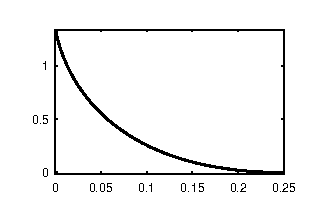
\includegraphics[width=5.5cm]{PDF/Logistic_var}} \caption{Entropy functional $\phi$ derived from the logistic distribution
with $T_{1}(x)=x^{2}$.}


\label{fig:Entropy-logistic-var}  & \centerline{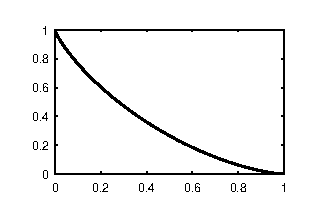
\includegraphics[width=5.5cm]{PDF/Logistic_moy}} \caption{Entropy functional $\phi$ ($\widetilde{\phi}_{\pm}=\pm\phi$) derived
from the logistic distribution with either partial moments $T_{\pm,1}(x)=x\un_{\X_{\pm}}(x)$,
or global moment $T_{1}(x)=x$.}


\label{fig:Entropy-logistic-moy} \tabularnewline
\end{tabular}
\end{figure}


% ---------- Arcsine



\subsection{The arcsine distribution}

\label{subsec:Arcsine}

The arcsine distribution is a special case of the beta distribution
with $\alpha=\beta=\frac{1}{2}$. We consider here the centered and
scaled version of this distribution which writes 
\[
f_{X}(x)=\frac{1}{\pi\sqrt{2\,\sigma^{2}-x^{2}}}\qquad\mbox{on}\qquad\X=(-\sigma\sqrt{2}\,;\,\sigma\sqrt{2}).
\]
The inverse distributions $f_{X,\pm}^{-1}$ on $\X_{-}=(-\sigma\sqrt{2}\,;\,0)$
and $X_{+}=[0\,;\,\sigma\sqrt{2})$ write then 
\[
f_{X,\pm}^{-1}(y)=\pm\frac{\sqrt{2\pi^{2}\sigma^{2}y^{2}-1}}{\pi y},\qquad y\ge\frac{1}{\pi\sigma\sqrt{2}}
\]


Let us now consider again either a second order moment as the constraint,
or (partial) first order moment(s).

% -- Arcsine - second order



\subsubsection{Second order moment}

When the second order moment $T_{1}(x)=x^{2}$ is constrained, one
immediately obtains 
\[
\phi'(y)=\lambda_{0}+\lambda_{1}\left(2\sigma^{2}-\frac{1}{\pi^{2}y^{2}}\right)
\]
With the special choice 
\[
\lambda_{0}=0\qquad\mbox{and}\qquad\lambda_{1}=1
\]
the entropy functional is then 
\[
\phi(y)=\left(2\sigma^{2}y+\frac{1}{\pi^{2}y}\right)\un_{\left[\frac{1}{\pi\sigma\sqrt{2}}\,;\,+\infty\right)}(y)
\]
which is represented figure~\ref{fig:Entropy-arcsin-var} for $\sigma=1$.

% ---------- Arcsine first order



\subsubsection{(Partial) first-order moment(s)}

Since the distribution does not share the sense of variation of $T_{1}(x)=x$,
either we turn out to consider it as an extremal distribution of an
entropy that is not concave, or as a maximum entropy when constraints
are of the type 
\[
T_{\pm,1}(x)=x\quad\mbox{over}\quad\X_{-}=\left(-\sigma\sqrt{2}\,;\,0\right),\quad\mbox{and}\quad\X_{+}=\left[0\,;\:\sigma\sqrt{2}\right).
\]
now 
\[
\phi_{\pm}'(y)=\lambda_{0}+\lambda_{\pm,1}\frac{\sqrt{2\pi^{2}\sigma^{2}y^{2}-1}}{\pi y}\qquad\mbox{or}\qquad\widetilde{\phi}_{\pm}'(y)=\lambda_{0}\pm\lambda_{1}\frac{\sqrt{2\pi^{2}\sigma^{2}y^{2}-1}}{\pi y}
\]
where the sign is absorbed in the factors $\lambda_{\pm,1}$. A judicious
choice can be 
\[
\lambda_{0}=0\qquad\mbox{and }\qquad\lambda_{\pm,1}=1\qquad\mbox{or}\qquad\lambda_{1}=1
\]
leading then either to the (convex) uniform function 
\[
\phi(y)=\left(\frac{1}{\pi}\sqrt{2\pi^{2}\sigma^{2}y^{2}-1}+\frac{1}{\pi}\arctan\left(\frac{1}{\sqrt{2\pi^{2}\sigma^{2}y^{2}-1}}\right)\right)\un_{\left[\frac{1}{\pi\sigma\sqrt{2}}\,;\,+\infty\right)}(y)
\]
or to the multiform function with branches $\widetilde{\phi}_{\pm}$,
\[
\widetilde{\phi}_{\pm}(y)=\pm\left(\frac{1}{\pi}\sqrt{2\pi^{2}\sigma^{2}y^{2}-1}+\frac{1}{\pi}\arctan\left(\frac{1}{\sqrt{2\pi^{2}\sigma^{2}y^{2}-1}}\right)\right)\un_{\left[\frac{1}{\pi\sigma\sqrt{2}}\,;\,+\infty\right)}(y)
\]


The uniform function is represented figure~\ref{fig:Entropy-arcsin-moy}
for $\sigma=1$ (here again $\widetilde{\phi}_{\pm}(y)=\pm\phi(y)$).

\
 
\begin{figure}[htbp]
\begin{tabular}{>{}m{.42\textwidth}>{}m{.58\textwidth}}
\centerline{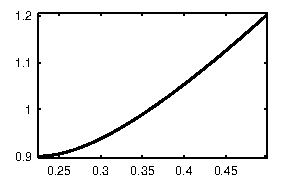
\includegraphics[width=5.5cm]{PDF/ArcsineCD_var}} \caption{Entropy functional $\phi$ derived from the centered and scaled arcsine
distribution with constraint $T_{1}=x^{2}$.}


\label{fig:Entropy-arcsin-var}  & \centerline{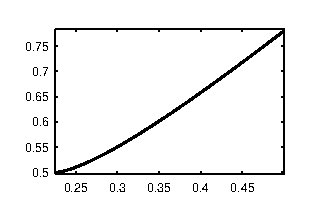
\includegraphics[width=5.5cm]{PDF/ArcsineCD_moy}} \caption{Entropy functional $\phi$ ($\widetilde{\phi}_{\pm}=\pm\phi$) derived
from the arcsine distribution either with partial constraints $T_{\pm,1}=x\un_{\X_{\pm}}(x)$,
or with global constraint $T_{1}(x)=x$.}


\label{fig:Entropy-arcsin-moy} \tabularnewline
\end{tabular}
\end{figure}


% ---------- Gamma first order



\subsection{The gamma distribution and (partial) first-order moment(s)}

\label{subsec:GammaFirstOrder}

As a very special case, consider here this distribution, expressed
as 
\[
f_{X}(x)=\frac{\beta^{\alpha}x^{\alpha-1}\exp(-\beta x)}{\Gamma(\alpha)}\qquad\mbox{on}\qquad\X=\Rset_{+}.
\]
Let us concentrate on the case $\alpha>1$ for which the distribution
is non-monotonous, unimodal, where the mode is located at $x=\frac{\alpha-1}{\beta}$
and $f_{X}(\Rset_{+})=\left[0\,;\,\frac{\beta}{\Gamma(\alpha)}\left(\frac{\alpha-1}{e}\right)^{\alpha-1}\right]$.
Thus, here again it cannot be viewed as a maximum entropy constraint
neither by the first order moment, nor by the second order moment.
Here, we can again interpret it as a maximum entropy constrained by
partial moments 
\[
T_{0,1}(x)=x^{i}\quad\mbox{over}\quad\X_{0}=\left[0\,;\,\frac{\alpha-1}{\beta}\right),\quad\mbox{and}\quad T_{-1,1}(x)=x^{i}\quad\mbox{over}\quad\X_{-1}=\left[\frac{\alpha-1}{\beta}\,;\:+\infty\right).
\]
or as an extremal entropy constrained by the moment 
\[
T_{1}(x)=x^{i}\quad\mbox{over}\quad\X=\Rset_{+}
\]
where $i=1$ or $i=2$. Inverting $y=f_{X}(x)$ leads to the equation
\[
\frac{\beta x}{1-\alpha}\exp\left(\frac{\beta x}{1-\alpha}\right)=-\frac{1}{\alpha-1}\left(\frac{\Gamma(\alpha)y}{\beta}\right)^{\frac{1}{\alpha-1}}
\]
to be solved. As expected, this equation has two solutions. These
solutions can be expressed via the multivalued Lambert-W function
$\W$ defined by $z=\W(z)\exp(\W(z))$, leading to the inverse functions
\[
f_{X,k}^{-1}(y)=\frac{\alpha-1}{\beta}\W_{k}\left(-\frac{1}{\alpha-1}\left(\frac{\Gamma(\alpha)y}{\beta}\right)^{\frac{1}{\alpha-1}}\right),\qquad y\in\left[0\,;\,\frac{\beta}{\Gamma(\alpha)}\left(\frac{\alpha-1}{e}\right)^{\alpha-1}\right],
\]
where $k$ denotes the branch of the Lambert-W function. $k=0$ gives
the principal branch and here it is related to the entropy part on
$\X_{0}$, while $k=-1$ gives the secondary branch, related to $\X_{-1}$
here.

% -- Gamma first order



\subsubsection{(Partial) first-order moment(s)}

In the context of the first order moment, $i=1$, one gets 
\[
\phi'_{k}(y)=\lambda_{0}+\frac{\alpha-1}{\beta}\lambda_{k,1}\W_{k}\left(-\frac{1}{\alpha-1}\left(\frac{\Gamma(\alpha)y}{\beta}\right)^{\frac{1}{\alpha-1}}\right)
\]
and similarly for $\widetilde{\phi}_{k}$ (with a unique $\lambda_{1}$
instead of the $\lambda_{k,1}$). To design a concave entropy, to
respect the sense of variation imposed on $\phi_{k}'(y)$, one can
choose 
\[
\lambda_{0}=0\qquad\mbox{and }\:\lambda_{k,1}\:\mbox{ such that}\qquad(-1)^{k+1}\,\lambda_{k,1}>0
\]
Indeed, there is no judicious choice allowing to compensate for the
asymmetry of $f_{X}$ and then allowing the definition of an uniform
function $\phi$. In general, there is no closed form for $\phi_{k}(y)$.
However, when $\alpha=2,\ldots$ is integer%
\footnote{Note that in this case, for $\beta=\frac{1}{2}$, $f_{X}$ is a chi-squared
distribution with $2\alpha$ degrees of freedom%
}, it can be checked that 
\[
\phi_{k}(y)=\frac{{\displaystyle (-1)^{k+1}\,\overline{\lambda}_{k,1}\: y\sum_{m=0}^{\alpha}\mu_{m}\left[\W_{k}\left(-\frac{1}{\alpha-1}\left(\frac{\Gamma(\alpha)y}{\beta}\right)^{\frac{1}{\alpha-1}}\right)\right]^{m}}}{\left[\W_{k}\left(-\frac{1}{\alpha-1}\left(\frac{\Gamma(\alpha)y}{\beta}\right)^{\frac{1}{\alpha-1}}\right)\right]^{\alpha-1}}\,+\, c_{k}
\]
where 
\[
\mu_{m}=\frac{(-1)^{\alpha-m}\,\Gamma(\alpha)}{\Gamma(m+1)\,(\alpha-1)^{\alpha-m}},\quad m=0,\ldots,\alpha-1,\quad\mbox{and}\quad\mu_{\alpha}=1
\]
% Voir avec des pochamer
$c_{k}$ is an integration constant and the multiplicative factor
is absorbed in the strictly positive $\overline{\lambda}_{k,1}$.
$\X_{-1}$ being unbounded, $c_{-1}$ is chosen to be zero and $c_{0}$
can be chosen such that $\phi_{k}\left(\frac{\beta}{\Gamma(\alpha)}\left(\frac{\alpha-1}{e}\right)^{\alpha-1}\right)$
coincide for instance. The same algebra leads to the same expression
for the $\widetilde{\phi}_{k}$, except that $(-1)^{k+1}\lambda_{k,1}$
are replaced by a unique $\lambda_{1}$.

The multivalued function $\phi$ in the concave context is represented
figure~\ref{fig:Entropy-gamma-moy} for $\beta=3$, $\alpha=2$ and
$\alpha=5$, and with the choices $\overline{\lambda}_{k,1}=1$ (for
the other context, with $\overline{\lambda}_{1}=-1$, $\widetilde{\phi}_{k}=(-1)^{k}\phi_{k}$.)
% = - \frac{2 \beta}{e}$.
\begin{figure}[htbp]
\centerline{ 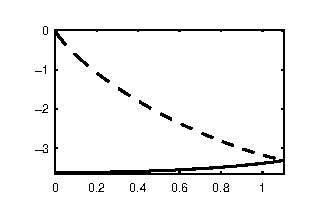
\includegraphics[width=5cm]{PDF/Gamma_2_moy} \hspace{2mm}
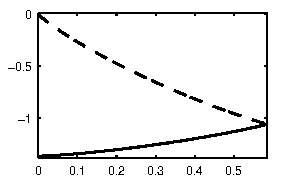
\includegraphics[width=5cm]{PDF/Gamma_5_moy}} \caption{Multiform entropy functional $\phi$ derived from the gamma distribution
with $\beta=3$, $T_{k,1}(x)=x\un_{\X_{k}}(x)$, $k\in\{0,-1\}$ (solid
line $\phi_{0}$ and dashed line $\phi_{-1}$). Left: $\alpha=2$;
Right: $\alpha=5$.}


\label{fig:Entropy-gamma-moy} 
\end{figure}


% (this choice is made to see each branch);
% \lambda_{0,1}   >  0 mais attention, phi_k' = - (a-1)/b W_k(-...)
% \lambda_{-1,1}  <   0


% ---------- Gamma second order



\subsubsection{(Partial) second-order moment(s)}

Now, we consider as constraints the (partial) second-order moment(s),
$i=2$. The same approach than in the previous case leads to 
\[
\phi'_{k}(y)=\lambda_{0}+\left(\frac{\alpha-1}{\beta}\right)^{2}\lambda_{k,1}\left[\W_{k}\left(-\frac{1}{\alpha-1}\left(\frac{\Gamma(\alpha)y}{\beta}\right)^{\frac{1}{\alpha-1}}\right)\right]^{2}
\]
To respect the sense of variation imposed on $\phi_{k}'(y)$, one
can choose again 
\[
\lambda_{0}=0\qquad\mbox{and }\:\lambda_{k,1}\:\mbox{ such that}\qquad(-1)^{k+1}\,\lambda_{k,1}>0
\]
and when $\alpha$ is integer ($\alpha\ge2$), it can be checked that
\[
\phi_{k}(y)=\frac{{\displaystyle (-1)^{k+1}\,\overline{\lambda}_{k,1}\: y\sum_{m=0}^{\alpha+1}\mu_{m}\left[\W_{k}\left(-\frac{1}{\alpha-1}\left(\frac{\Gamma(\alpha)y}{\beta}\right)^{\frac{1}{\alpha-1}}\right)\right]^{m}}}{\left[\W_{k}\left(-\frac{1}{\alpha-1}\left(\frac{\Gamma(\alpha)y}{\beta}\right)^{\frac{1}{\alpha-1}}\right)\right]^{\alpha-1}}\,+\, c_{k}
\]
where 
\[
\mu_{m}=\frac{2\,(-1)^{\alpha-m+1}\,\Gamma(\alpha+1)}{\Gamma(m+1)\,(\alpha-1)^{\alpha-m+1}},\quad m=0,\ldots,\alpha,\quad\mbox{and}\quad\mu_{\alpha+1}=1
\]
% Voir avec des pochamer
and $c_{k}$ is an integration constant and the multiplicative factor
is absorbed in the strictly positive $\overline{\lambda}_{k,1}$.
Again $c_{-1}$ is chosen to be zero and $c_{0}$ can be chosen such
that $\phi_{k}\left(\frac{\beta}{\Gamma(\alpha)}\left(\frac{\alpha-1}{e}\right)^{\alpha-1}\right)$
coincide. This multivalued function is represented figure~\ref{fig:Entropy-gamma-var}
for $\beta=3$, $\alpha=5$ and $\alpha=10$, and with the choices
$\overline{\lambda}_{k,1}=1$ % = - \frac{2 \beta}{e}$.
\begin{figure}[htbp]
\centerline{ 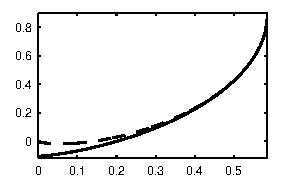
\includegraphics[width=5cm]{PDF/Gamma_5_var} \hspace{2mm}
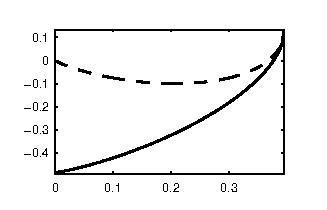
\includegraphics[width=5cm]{PDF/Gamma_10_var}} \caption{Multiform entropy functional $\phi$ derived from the gamma distribution
with $\beta=3$, $T_{k,1}(x)=x^{2}\un_{\X_{k}}(x)$, $k\in\{0,-1\}$
(solid line $\phi_{0}$ and dashed line $\phi_{-1}$). Left: $\alpha=5$;
Right: $\alpha=10$.}


\label{fig:Entropy-gamma-var} 
\end{figure}


Here again, the approach with a global constraint $T_{1}(x)=x^{2}$
over $\X=\Rset_{+}$, with the choice $\overline{\lambda}_{1}=-1$,
leads simply to $\widetilde{\phi}_{k}=(-1)^{k}\phi_{k}$. % (this choice is made to see each branch);
% \lambda_{0,1}   >  0 mais attention, phi_k' = - (a-1)/b W_k(-...)
% \lambda_{-1,1}  <   0


%%%%%%%%%%%%%%%%%%%%%%%%%%%%%%%%%


\vspace{1cm}


\centerline{\underline{\hspace{10cm}}}

\vspace{1cm}


% ---------- q-Normal


%\subsection{Hyperbolic secant distribution and first-order moment}


Let us consider some specific cases. 
\begin{enumerate}
\item Let $f_{X}(x)$ be the hyperbolic nt distribution, with density 
\[
f_{X}(x)=\frac{1}{2}\text{sech}(\frac{\pi}{2}x)=\frac{1}{2}\cosh^{-1}(\frac{\pi}{2}x).
\]
Obviously, $\frac{\pi}{2}x=\cosh(2y)=\phi'(y)$ with $T(x)=x$, $\lambda=\frac{\pi}{2}$,
and 
\[
\phi(y)=\sinh(2y).
\]
So doing, we obtain an hyperbolic sine entropy with the hyperbolic
secant distribution as the associated maximum entropy distribution. 
\end{enumerate}
{document} 
\end{document}
